\documentclass[10pt]{article}
\usepackage[a4paper,margin=1.0cm]{geometry}
\usepackage{tikz}
\usepackage{pgfplots}
\pgfplotsset{compat=1.18}
\usetikzlibrary{arrows.meta,positioning,shapes.geometric}
\usepackage{xcolor}
\usepackage{enumitem}
\usepackage{multicol}
\usepackage{titlesec}
\usepackage[hidelinks]{hyperref}

\definecolor{nbblue}{HTML}{1F4E79}
\definecolor{nbteal}{HTML}{2E8B8B}
\definecolor{nbred}{HTML}{C0392B}
\definecolor{nbgrey}{HTML}{595959}

\setlength{\parindent}{0pt}
\setlength{\parskip}{2pt}
\titlespacing{\section}{0pt}{4pt}{2pt}
\titleformat{\section}{\normalfont\bfseries\color{nbblue}\small}{}{0pt}{}
\setlist[itemize]{leftmargin=1.1em,itemsep=0pt,topsep=1pt,parsep=0pt}
\pagestyle{empty}

\newcommand{\hd}[1]{{\color{nbblue}\textbf{#1}}}

\begin{document}
\small

%==================== TITLE ====================
\begin{center}
{\Large\bfseries\color{nbblue} The Edge Negotiator}\\[1pt]
{\bfseries Verified-Source Cross-Junction Coordination for SLM-Driven Traffic Signal Control}\\[2pt]
{\footnotesize Progress report $\cdot$ UCL MSc Systems Engineering for IoT (25153651) $\cdot$ Supervisors: Dr A.\ Delibasi (UCL), L.\ Stott (Microsoft) $\cdot$ 2026-06-20}
\end{center}
\vspace{-4pt}
\hrule height 1pt
\vspace{4pt}

%==================== SCOPE ====================
\section{1.\ The project and its goal}
The system is a corridor of traffic junctions on one arterial. Each junction runs a fast classical controller (\emph{MaxPressure}$^{[1]}$) by default, which is also the safety floor. Alongside it runs a small AI model (\textbf{Phi-4-mini}, on the junction itself via \textbf{Microsoft Foundry Local}, never retrained), called in only for hard cases. Junctions share what they are about to do over a channel that is digitally signed and checked for plausibility.

The goal: coordinate well in normal traffic, and fail safely when a neighbour lies. If a junction's messages are tampered with or the junction is hijacked, the system detects that the reports do not match reality and falls back to local control. A deterministic safety net always makes the clear-cut calls: clear an ambulance a junction can physically detect, refuse a claim it cannot verify; safety never depends on the AI. The AI handles only what a fixed rule cannot settle: when an alert is flagged but the evidence is partial or conflicting, it weighs the neighbours' reports to judge a real incident from a spoofed grab. Whether that beats a well-tuned fixed rule is the central question we measure, and we report it either way.

%==================== TWO COLUMNS: diagram + chart ====================
\vspace{2pt}
\begin{minipage}[t]{0.50\textwidth}
\section{2.\ How it works}
\centering
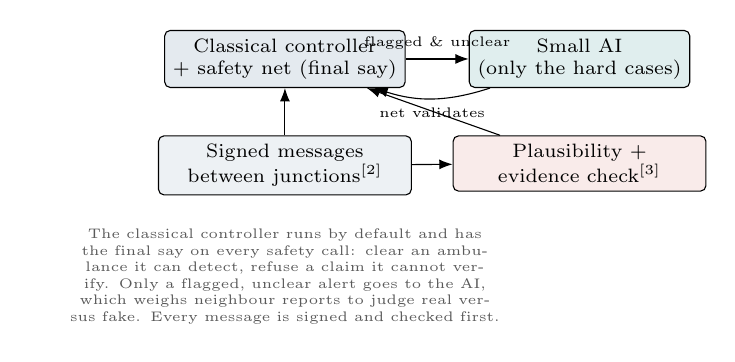
\begin{tikzpicture}[
  font=\scriptsize,
  box/.style={draw,rounded corners=2pt,align=center,inner sep=3pt,minimum height=7mm},
  >=Latex]
\node[box,fill=nbblue!12] (mp) {Classical controller\\+ safety net (final say)};
\node[box,fill=nbteal!15,right=8mm of mp] (slm) {Small AI\\(only the hard cases)};
\node[box,fill=nbblue!8,below=6mm of mp,text width=3.0cm] (bus) {Signed messages\\between junctions$^{[2]}$};
\node[box,fill=nbred!10,below=6mm of slm,text width=3.0cm] (gate) {Plausibility +\\evidence check$^{[3]}$};
\draw[->] (mp) -- node[above,font=\tiny]{flagged \& unclear} (slm);
\draw[->] (slm) to[bend left=18] node[below,font=\tiny]{net validates} (mp);
\draw[->] (bus) -- (mp);
\draw[->] (bus) -- (gate);
\draw[->] (gate) -- (mp);
\node[below=3mm of bus,font=\tiny,text width=6.3cm,align=center,color=nbgrey]
  {The classical controller runs by default and has the final say on every safety call: clear an ambulance it can detect, refuse a claim it cannot verify. Only a flagged, unclear alert goes to the AI, which weighs neighbour reports to judge real versus fake. Every message is signed and checked first.};
\end{tikzpicture}
\end{minipage}\hfill
\begin{minipage}[t]{0.47\textwidth}
\section{3.\ Measured effects (30 runs each)}
\centering
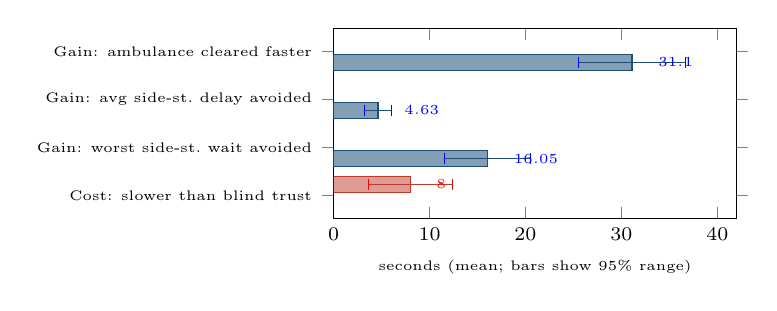
\begin{tikzpicture}
\begin{axis}[
  width=6.7cm,height=4.0cm,font=\scriptsize,
  xbar,xmin=0,xmax=42,
  bar width=6pt,
  enlarge y limits=0.16,
  xlabel={seconds (mean; bars show 95\% range)},
  xlabel style={font=\tiny},
  ytick={0,1,2,3},
  yticklabels={Cost: slower than blind trust,Gain: worst side-st.\ wait avoided,Gain: avg side-st.\ delay avoided,Gain: ambulance cleared faster},
  yticklabel style={font=\tiny,align=right},
  nodes near coords,nodes near coords style={font=\tiny},
  every node near coord/.append style={xshift=6pt}]
\addplot+[draw=nbblue,fill=nbblue!55,
  error bars/.cd,x dir=both,x explicit] coordinates {
  (16.05,1)+-(4.47,0)
  (4.63,2) +-(1.37,0)
  (31.1,3) +-(5.55,0)};
\addplot+[draw=nbred,fill=nbred!50,
  error bars/.cd,x dir=both,x explicit] coordinates {
  (8.0,0)  +-(4.39,0)};
\end{axis}
\end{tikzpicture}\\[-1pt]
{\scriptsize SUMO$^{[4]}$, 30 paired runs. Gains (blue) are versus the no-defence baselines: no preemption, or trust-everything under attack. The cost (red) is versus blindly trusting. Every 95\% range excludes zero.}
\end{minipage}

%==================== PROGRESS ====================
\vspace{1pt}
\section{4.\ What we have built}
\begin{multicols}{2}
\begin{itemize}
\item \hd{Working and tested:} signed messaging between junctions, an approved-senders registry, the classical controller and its safety net, a check that flags neighbour reports inconsistent with the traffic actually on the road, and a four-junction simulated corridor.
\item \hd{Emergency handling:} a junction clears an ambulance only with physical evidence the vehicle exists. A valid signature is not enough, so a faked emergency is refused.
\item \hd{Attack-and-defence demo (runs live):} a hijacked junction sends a signed but fake ``ambulance approaching'' alert and it is refused; a real ambulance is cleared at every junction. Measured against a trust-everything controller and the plain classical controller.
\item \hd{Evidence (30 runs, Section 3):} with emergency handling the ambulance clears 31\,s faster than with none. Under the spoof attack our system holds the worst side-street wait 16\,s below the trust-everything controller. Requiring evidence costs 8\,s of ambulance time versus blindly trusting, a price we accept.
\item \hd{Independent check:} an automated audit of our written specification found no fabricated sources; a few over-stated citations were corrected. Every result is reproducible from its settings.
\end{itemize}
\end{multicols}

%==================== NOVELTY ====================
\vspace{-2pt}
\section{5.\ What is new}
To our knowledge, no prior system has been evaluated as a multi-junction, AI-coordinated controller in which a junction's messages can be \emph{faked by an insider that still holds a valid key}. The individual parts exist; the combination, tested under that threat, does not. Nearest work: \textbf{CoLLMLight}$^{[5]}$ (AI junctions coordinate, but trust each other completely); \textbf{VLMLight}$^{[6]}$ (fast-classical plus slow-AI, single junction, very large models, no trust); \textbf{LA-Light}$^{[7]}$ (AI for rare events, cloud-based, no malicious faults); \textbf{Keijzer\,2021}$^{[8]}$ (detects coordination attacks, but only in theory, with no measurement against attacker strength). Our contribution: a small on-device AI, a \emph{measured} curve of how detection holds up as the attack grows, verifiable identity, and a tamper-proof log.

%==================== NEXT ====================
\section{6.\ Next steps}
\begin{multicols}{2}
\begin{itemize}
\item \hd{Central experiment:} on flagged, unclear alerts, does the AI beat a well-tuned fixed rule? Measure it; report it either way, including a null.
\item Larger evaluation: more demand levels and a real London (Lambeth) arterial, with many paired runs and confidence ranges.
\item Detection limit: increase the size of the lie until detection fails, and report where that point is.
\item Heavier traffic, where the preemption benefit and the attack damage are largest.
\item Run the real Phi-4-mini on Foundry Local and confirm its decisions are repeatable.
\end{itemize}
\end{multicols}

%==================== HONESTY ====================
\vspace{-1pt}
\section{7.\ What we do and do not claim}
{\footnotesize \textbf{We claim:} authenticated messaging between junctions; detection of faked or faulty neighbour reports with a measured reliability curve; a deterministic safety floor; and a fair attack-and-defence comparison. \textbf{We do not claim:} new cryptography; that the AI beats the classical controller on ordinary traffic; that the AI yet improves the hard, ambiguous decisions (measured next); defence against two or more junctions colluding, or against a stolen master key; or that simulator results transfer directly to real hardware (future work).}

%==================== REFS ====================
\vspace{2pt}
\hrule
\vspace{2pt}
{\scriptsize\color{nbgrey}
\textbf{References.}
[1] Varaiya, Max-pressure control, \emph{Transp.\ Res.\ C} 36 (2013).
[2] Bernstein et al., Ed25519, \emph{J.\ Cryptogr.\ Eng.} (2012).
[3] Lighthill \& Whitham, \emph{Proc.\ R.\ Soc.\ A} 229 (1955); Richards, \emph{Oper.\ Res.} 4 (1956) (vehicle-conservation law).
[4] Lopez et al., SUMO, \emph{IEEE ITSC} (2018).
[5] Yuan et al., CoLLMLight, arXiv:2503.11739 (2025).
[6] Wang et al., VLMLight, arXiv:2505.19486 (2025).
[7] Wang et al., LA-Light, arXiv:2403.08337 (2024).
[8] Keijzer et al., collaborative-intersection attack detection, \emph{ECC} (2021).
}
\end{document}
